\section{Zadanie 3}
\subsection{II norma macierzowa - charakterystyka i porównanie}

Druga norma macierzowa (norma spektralna) jest zdefiniowana jako największa wartość singularna macierzy \( A \). Oznacza to, że odpowiada pierwiastkowi największej wartości własnej macierzy \( A^T A \), co pozwala efektywnie ocenić rozkład wartości w macierzy.

W naszym algorytmie obliczenia tej normy opierają się na wyznaczaniu miejsc zerowych wielomianu charakterystycznego macierzy. Jednak takie podejście jest wrażliwe na błędy numeryczne, szczególnie w przypadku macierzy o bliskich sobie wartościach własnych. Operacje na pierwiastkach wielomianu mogą prowadzić do niepożądanych efektów, takich jak pojawianie się zespolonych wartości błędów wynikających z zaokrągleń lub niestabilności obliczeń.

Standardowo do wyznaczania II normy macierzowej można wykorzystać \textit{metodę potęgową}. Jest to iteracyjna technika, która pozwala na stabilne przybliżenie największej wartości własnej macierzy. W tej metodzie:
\begin{enumerate}
    \item Rozpoczynamy od wektora \( v_0 \) o dowolnych wartościach.
    \item W każdej iteracji obliczamy \( v_{k+1} = Av_k \) i normalizujemy wynikowy wektor.
    \item Proces powtarzamy, aż kolejne iteracje przyniosą zbieżność do wartości własnej odpowiadającej największej wartości absolutnej.
\end{enumerate}
Metoda ta jest bardziej stabilna niż operacje na wielomianie charakterystycznym, ponieważ unika problemów związanych z błędami zaokrągleń oraz nie wymaga wyznaczania pierwiastków. 

\subsection{Wyniki i wnioski:}

Porównując naszą funkcję \( \text{norm2} \) z wbudowaną w Octave funkcją \( \text{norm} \), obserwujemy rozbieżności wynikające z błędów numerycznych. Nasza implementacja wykazuje większe wrażliwości na błędy związane z obliczaniem pierwiastków wielomianu charakterystycznego, szczególnie w przypadku macierzy o zbliżonych wartościach własnych. Ponadto, dla macierzy o dużych wartościach na przekątnej mogą występować błędy wynikające z zaokrągleń spowodowanych ograniczoną precyzją operacji arytmetycznych.

Dla lepszego zilustrowania błędów w naszej implementacji mamy rozpisany wykres. 

\centering 
\begin{minipage}{0.6\textwidth}
    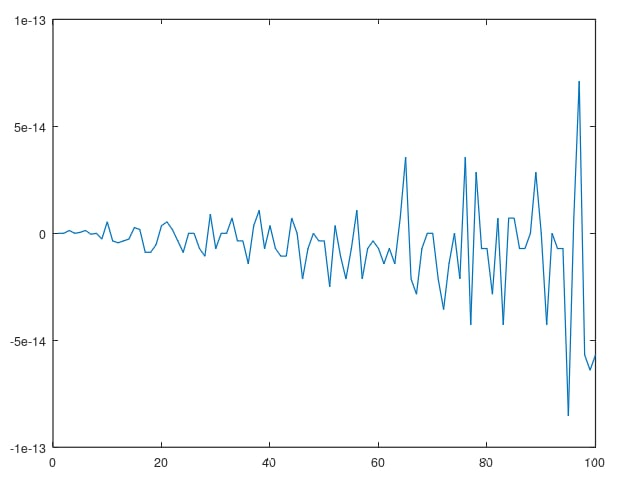
\includegraphics[width=\textwidth]{wykresy/zadanie3_blad.jpg}
\end{minipage}

\textbf{Wnioski:}
\begin{itemize}
    \item Widzimy że otrzymujemy bardzo duże wachania związane z błędem. Algorytm jest niestabilny numerycznie.
\end{itemize}
